%% Put these somewhwere:

\XXX{use svalue(g), spacing to give some breathing room in a ggroup}

\XXX{something like ggroup(cont=w,spacing=10); svalue(g)=10}

\XXX{include listing data frame, listing variables by type}

\XXX{relationship with the toolkits

\XXX{getToolkitWidget, add method, ... only with RGtk2 (rJava?), only some widgets}}



%% gWidgets introduction
 
\newcommand{\ONLYIN}[1]{[only in #1]}

\chapter{\pkg{gWidgets}: Overview}
\label{sec:overview}

%% Overview of gWidgets

% ML: do we really want to discuss the unsupported rJava backend?
% I am also confused about gWidgetsWWW - is it an implementation or
% something that just resembles the gWidgets API?

% JV, I will drop rJava, put in gWidgetsQt, and make brief mention of gWidgetsWWW

The \pkg{gWidgets} package provides a toolkit-independent interface
for the \R\/ user to program graphical user interfaces from within
R. Although the package provides much less functionality than using a
native toolkit interface, \pkg{gWidgets} can be used to create
moderately complex GUIs quickly and easily using a programming
interface that is simpler and more familiar to the \R\/ user.

Figure~\ref{fig:gWidgets-three-oses} demonstrates the portability of
\pkg{gWidgets} commands, as it shows realizations on different
operating systems and with different graphical toolkits.

\begin{figure}
  \centering
  \begin{tabular}{ll}
    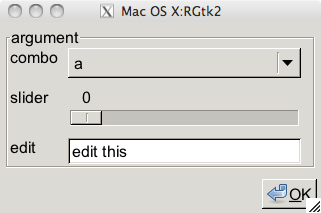
\includegraphics[width=0.45\textwidth]{ex-33-macosx-rgtk2} &
    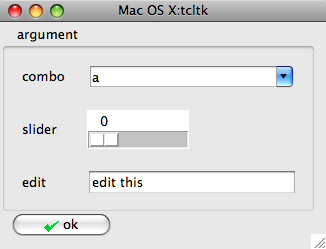
\includegraphics[width=0.45\textwidth]{fig-gWidgets-ex-33-tlctk}\\
    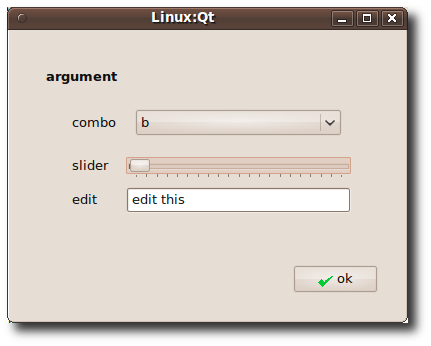
\includegraphics[width=0.45\textwidth]{ex-33-linux-qt} &
    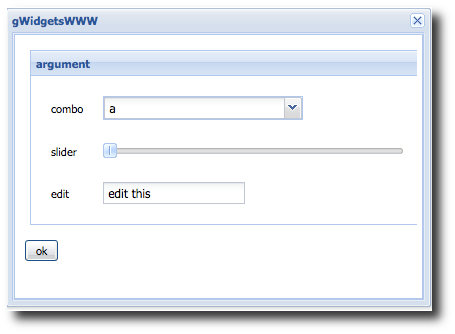
\includegraphics[width=0.45\textwidth]{ex-33-gWidgetsWWW}
  \end{tabular}
  \caption{The \pkg{gWidgets} package works with different operating
    systems and different GUI toolkits. This shows, the same code using the
    \pkg{RGtk2}, \pkg{tcltk}, \pkg{qtbase} packages for a toolkit. Additionally,
    the \pkg{gWidgetsWWW} package is used in the lower right figure.}
  \label{fig:gWidgets-three-oses}
\end{figure}

% %% Make figure -- work on layout here
% \XXX{Do mac, windows}
% \begin{figure}
%   \centering
%   \begin{tabular}{lccc}
%     & \pkg{RGtk2} & \pkg{tcltk} & \pkg{rJava} 
%     \\
%     L &
%     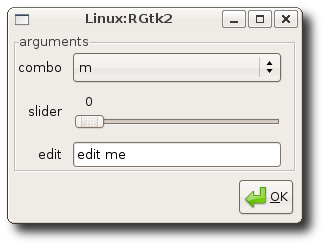
\includegraphics[width=0.3\textwidth]{ex-33-linux-rgtk2.png} &
%     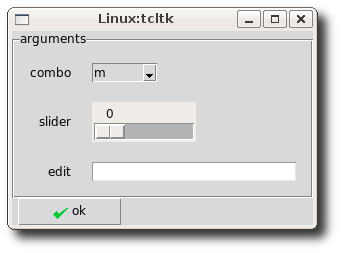
\includegraphics[width=0.3\textwidth]{ex-33-linux-tcltk} &
%     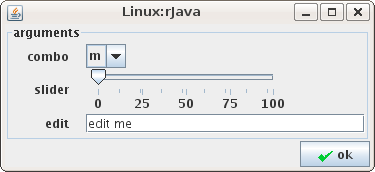
\includegraphics[width=0.3\textwidth]{ex-33-linux-rJava} 
%     \\
%     W &
%     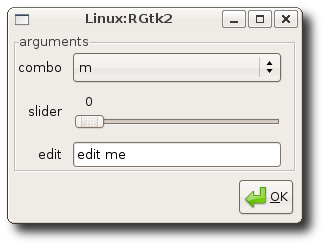
\includegraphics[width=0.3\textwidth]{ex-33-linux-rgtk2} &
%     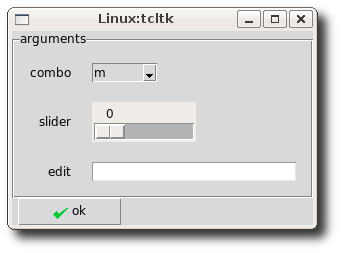
\includegraphics[width=0.3\textwidth]{ex-33-linux-tcltk} &
%     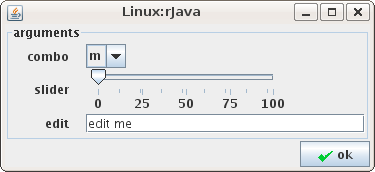
\includegraphics[width=0.3\textwidth]{ex-33-linux-rJava} 
%     \\
%     Mac &
%     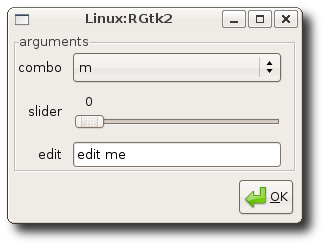
\includegraphics[width=0.3\textwidth]{ex-33-linux-rgtk2} &
%     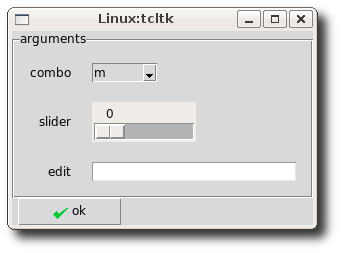
\includegraphics[width=0.3\textwidth]{ex-33-linux-tcltk} &
%     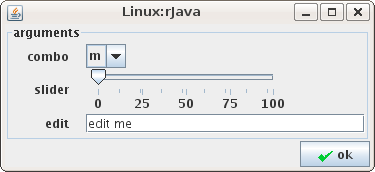
\includegraphics[width=0.3\textwidth]{ex-33-linux-rJava}
%   \end{tabular}
%   \caption{The \pkg{gWidgets} package works with different operating systems and different GUI toolkits. This shows the combination of \code{linux}, \code{Mac OS X (10.5)} and \code{Windows XP} and the packages \pkg{RGtk2}, \pkg{tcltk}, and \pkg{rJava}}
%   \label{fig:three-oses-three-toolkits}
% \end{figure}


% \begin{figure}
%   \centering
%   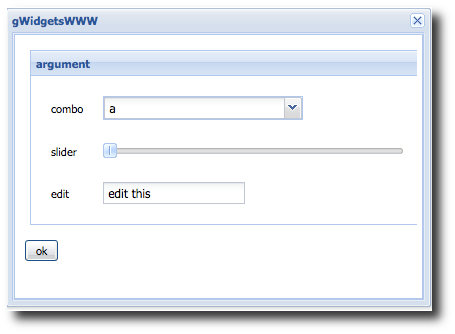
\includegraphics[width=.45\textwidth]{ex-33-gWidgetsWWW}
%   \caption{A GUI shown using \pkg{gWidgetsWWW}.}
%   \label{fig:gWidgetsWWW-same-gui}
% \end{figure}





\section{Constructors}
\label{sec:constructors}

We begin with some sample \pkg{gWidgets} commands that set up a basic
interface allowing a user to input some test. The first line loads the
package, the others will be described later.

\begin{Schunk}
\begin{Sinput}
 require(gWidgets)
 options(guiToolkit="RGtk2")
 w <- gwindow("Text input example", visible=FALSE)